\documentclass[a4paper,notitlepage,parskip=half]{scrartcl}

\usepackage{color}
\usepackage{ngerman}
\usepackage{graphicx}
\areaset[1cm]{16cm}{26cm}
\usepackage{float}
\usepackage{fancybox}
\usepackage[T1]{fontenc}
\usepackage[utf8]{inputenc}
\usepackage{pifont}
\usepackage{url}
\usepackage{booktabs}
\usepackage{amsmath}
\usepackage{listingsutf8}
\usepackage[german]{varioref}
\usepackage{colortbl} % Farbige Tabellen
\usepackage{tabularx} % Mehrzeilige Tabellenzellen (nicht benutzt)
\usepackage{longtable}
%\usepackage[german,scrtime,time]{prelim2e}
%\usepackage{svn}
\usepackage{marginnote}
\usepackage{xcolor}
\graphicspath{{./jpg/}}
\DeclareGraphicsExtensions{.jpg,.eps,.png}
%\usepackage{courier}

\usepackage[most]{tcolorbox}
\usepackage{tikz}
\usetikzlibrary{intersections}
\usetikzlibrary{
  arrows,
  decorations.pathreplacing,
  shapes.symbols
}

% Wenn pdflatex benutzt wird sollen die 
% installierten! frutiger-Fonts verwendet werden
% Ansonsten cmbright
\Ifpdfoutput %
{%
\usepackage[scaled=0.90]{frutiger}
\renewcommand\familydefault{\sfdefault}
%\DeclareFixedFont\ott{T1}{phv}{mc}{n}{10pt
}%
{%
\usepackage{cmbright}
}%

\newcommand*\circled[1]{\tikz[baseline=(char.base)]{
            \node[shape=circle,draw,inner sep=2pt] (char) {#1};}}

\newtcbox{\button}[1][yellow]{on line,
arc=3pt,colback=#1!5!white,colframe=#1!20!black,
before upper={\rule[-2pt]{0pt}{10pt}},boxrule=1pt,
boxsep=0pt,left=2pt,right=2pt,top=1pt,bottom=.5pt}


% falls man das auch noch ändern möchte
\newcommand{\pihk}{PIHK\ }
\newcommand{\titel}{PIHK}
\newcommand{\vnr}{3.0.6}

%\newcommand{\ffile}[1]{\par\centerline{\tt#1}\par}
\newcommand{\ffile}[1]{{\texttt{#1}}}
\newcommand{\cfile}[1]{{\texttt{#1}}}
\newcommand{\ttctable}[1]{\centerline{\texttt{#1}}}
\newcommand{\sname}[1]{\emph{#1}}
\definecolor{listinggray}{gray}{0.95}
\definecolor{OliveGreen}{rgb}{0,0.5,0}
\definecolor{pastellblau}{rgb}{0.85,0.95,1.0} 

\newcolumntype{g}{>{\columncolor{pastellblau}}l}

\lstset{literate=%
  {Ö}{{\"O}}1
  {Ä}{{\"A}}1
  {Ü}{{\"U}}1
  {ß}{{\ss}}1
  {ü}{{\"u}}1
  {ä}{{\"a}}1
  {ö}{{\"o}}1
}
\lstset{numbers=left,numbersep=5pt,numberstyle=\tiny,%
    frame=none,basicstyle=\scriptsize\ttfamily,breaklines=true,%
    captionpos=b,backgroundcolor=\color{listinggray},frame=single}

% \parindent0cm
% \parskip1ex
\setlength{\parindent}{0em}


%\usepackage{courier}
\newtcolorbox{marker}[1][]{enhanced,
  before skip=2mm,after skip=3mm,
  boxrule=0.4pt,left=5mm,right=2mm,top=1mm,bottom=1mm,
  colback=yellow!50,
  colframe=yellow!20!black,
  sharp corners,rounded corners=southeast,arc is angular,arc=3mm,
  underlay={%
    \path[fill=tcbcolback!80!black] ([yshift=3mm]interior.south east)--++(-0.4,-0.1)--++(0.1,-0.2);
    \path[draw=tcbcolframe,shorten <=-0.05mm,shorten >=-0.05mm] ([yshift=3mm]interior.south east)--++(-0.4,-0.1)--++(0.1,-0.2);
    \path[fill=yellow!50!black,draw=none] (interior.south west) rectangle node[red!20!white]{\Huge\bfseries !} ([xshift=4mm]interior.north west);
    },
  drop fuzzy shadow,#1}


\begin{document}

\titlehead{\centerline{Frank Zimmermann \ding{70} Software \ding{70} Tools }}
% %\titlehead{\includegraphics{zenlogo}}
% \subject{Dokumentation}

\title{\begin{center}

\includegraphics[width=3.2cm]{myLogoPIHK3a.png}
\end{center}PIHK\\{\small Version \vnr}}
\subtitle{Programm zur Unterstützung bei IHK--Prüfungen\\[2ex]{\small Letztes Änderungsdatum:  \today} }
\author{Frank Zimmermann\\[0.5ex]{\small fz@zenmeister.de}}
\date{\small Erstellungsdatum: 20.06.2016}
\maketitle

\begin{abstract}
\setlength{\parindent}{0em}
Diese Dokumentation beschreibt das Programm \pihk in der Version \vnr.\\ 
\end{abstract}

\begin{figure}[ht]
    \centering
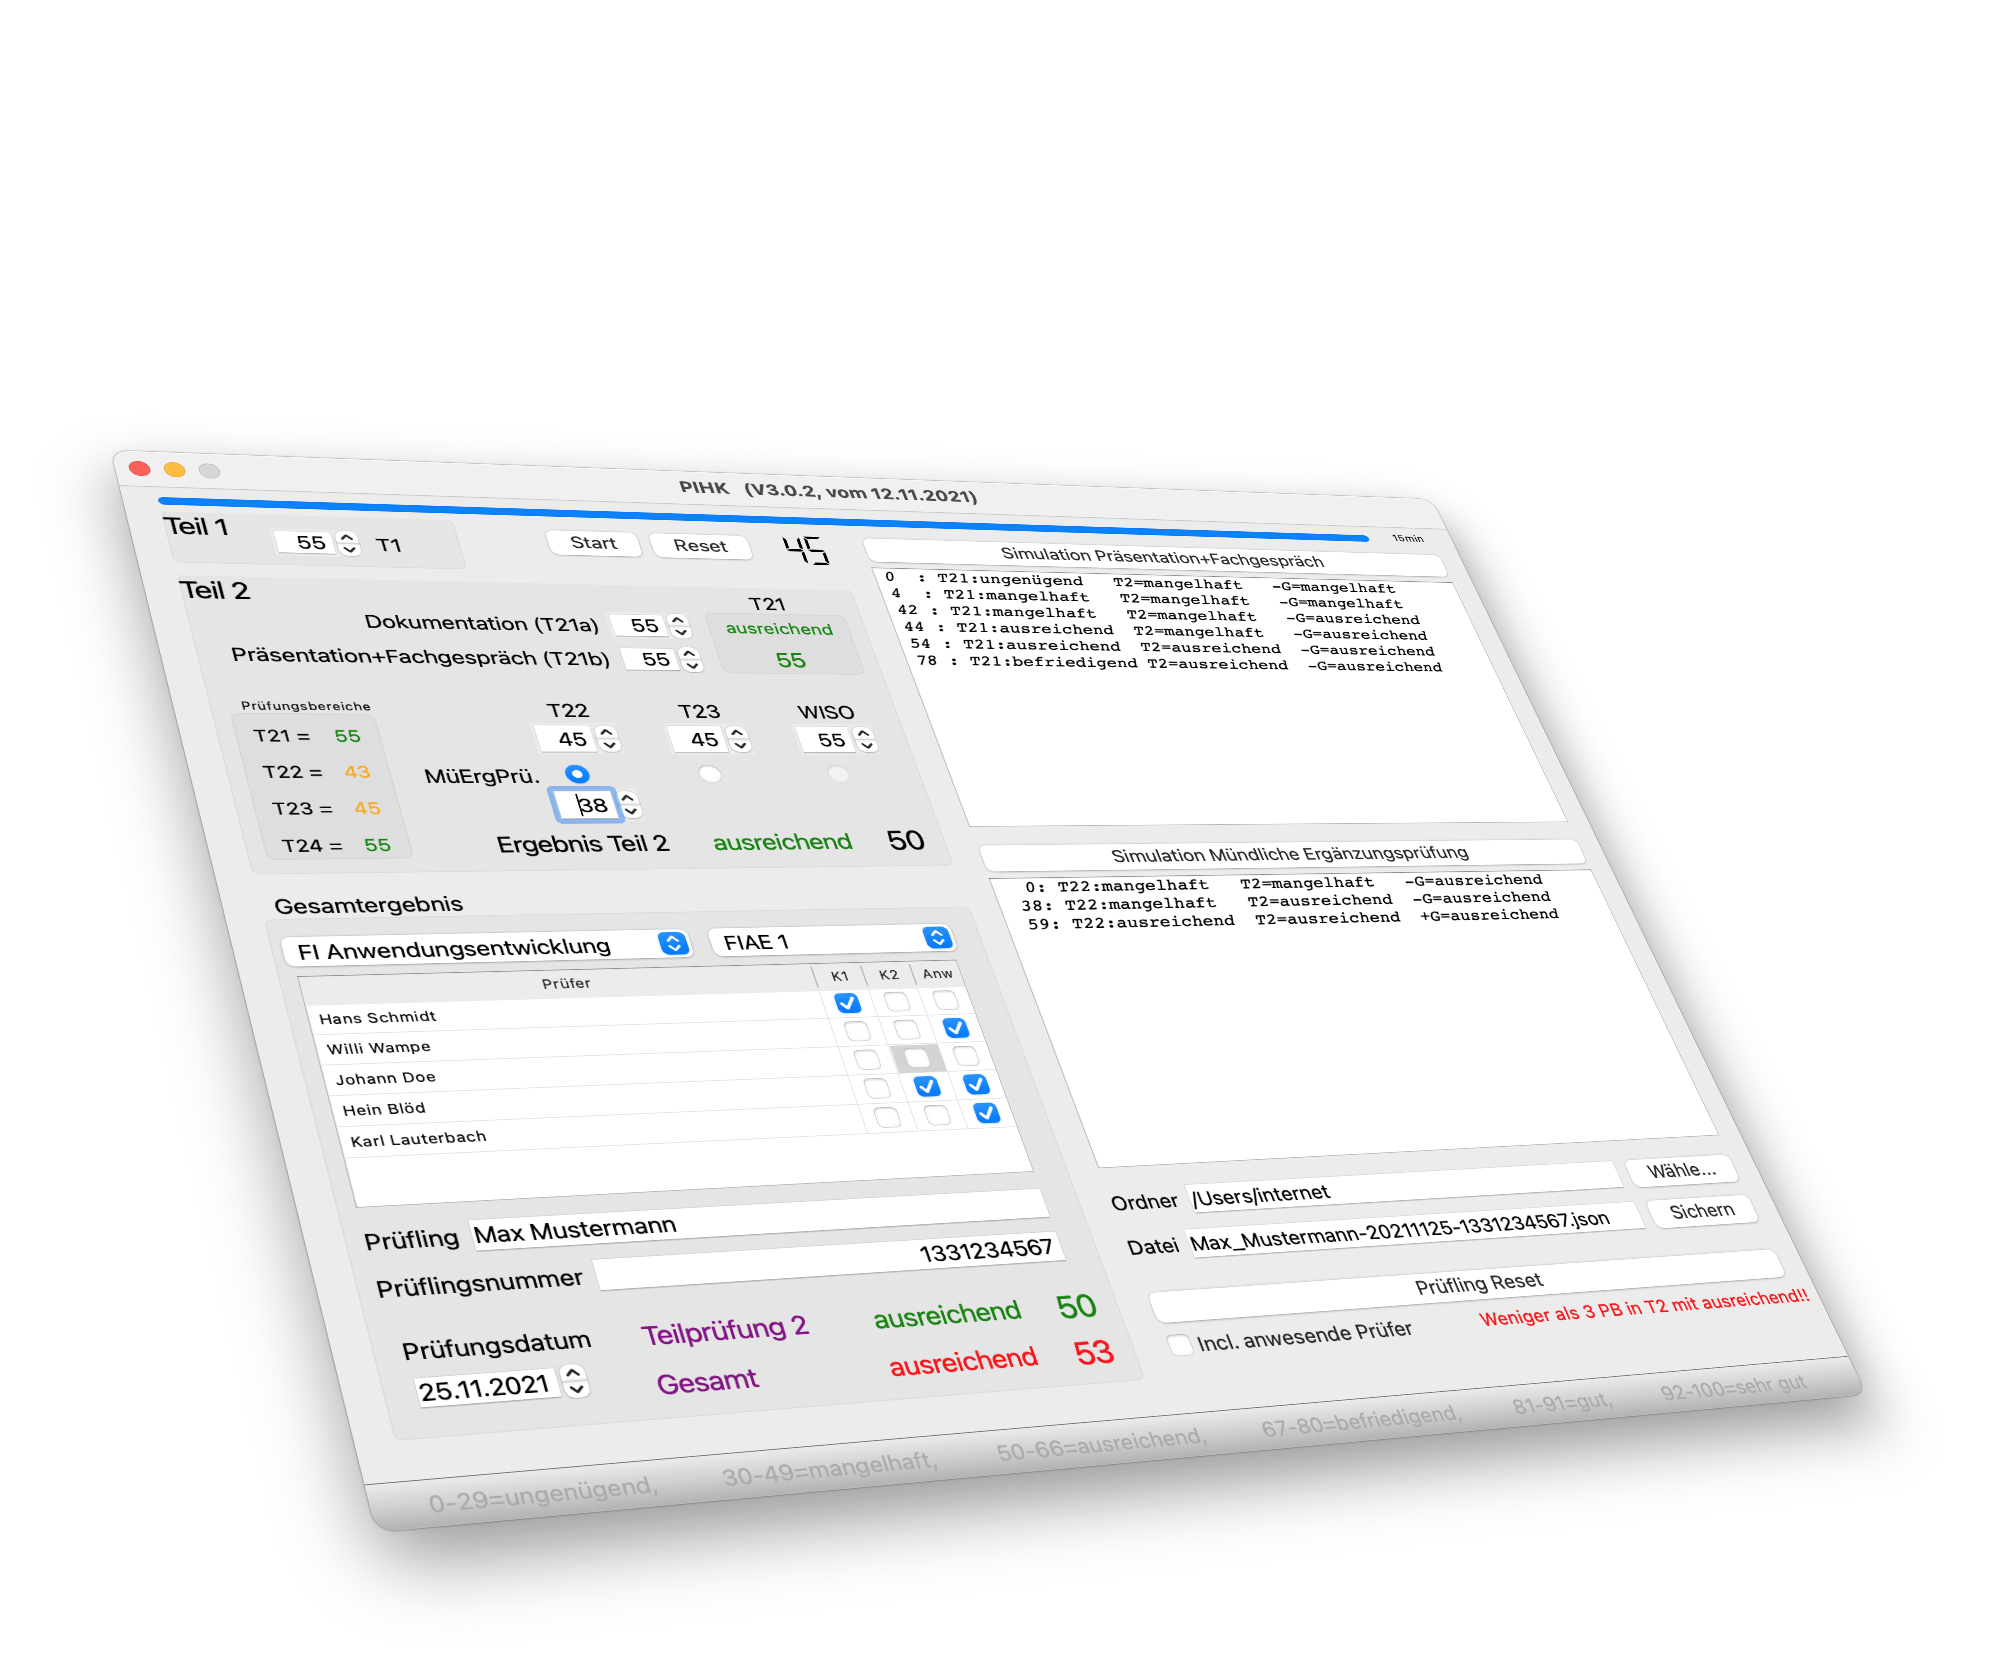
\includegraphics[width=15cm]{frontbild.png}
    %\caption{Programm für IHK Prüfungen}
    \label{fig:programm}
\end{figure}

\newpage
\rule{\linewidth}{1pt}
\tableofcontents
\rule{\linewidth}{1pt}

\newpage

\section{Motivation}
Das Programm \pihk wurde geschrieben, um bei IHK--Prüfungen der Fachinformatiker
bei der IHK--Hannover eine Hilfe bei der Berechnung und Vergabe der Punkte zu sein. Dabei wurden die 
Regularien der IHK--Hannover zugrunde gelegt. Eine Verwendung bei anderen Prüfungen
ist natürlich möglich, sofern die Regularien zur Berechnung identisch sind.
Die genauen Regularien stammen aus dem Dokument:

\begin{quote}
\emph{Verordnung über die Berufsausbildung im Bereich der Informations-- und Telekommunikationstechnik  (veröffentlicht im Bundesgesetzblatt Teil I Nr. 9 vom 05. März 2020)}
\end{quote}

\section{Neue Prüfungordnung}
Die neue Prüfungsordnung gliedert die Ausbildung neu und sieht eine etwas andere Berechnungsart vor, in der die Gewichtungen 
und die Prüfungsbereiche verändert wurden  (siehe dazu Abbildung~\ref{fig:berechnung}).

\begin{figure}[ht]
    \centering
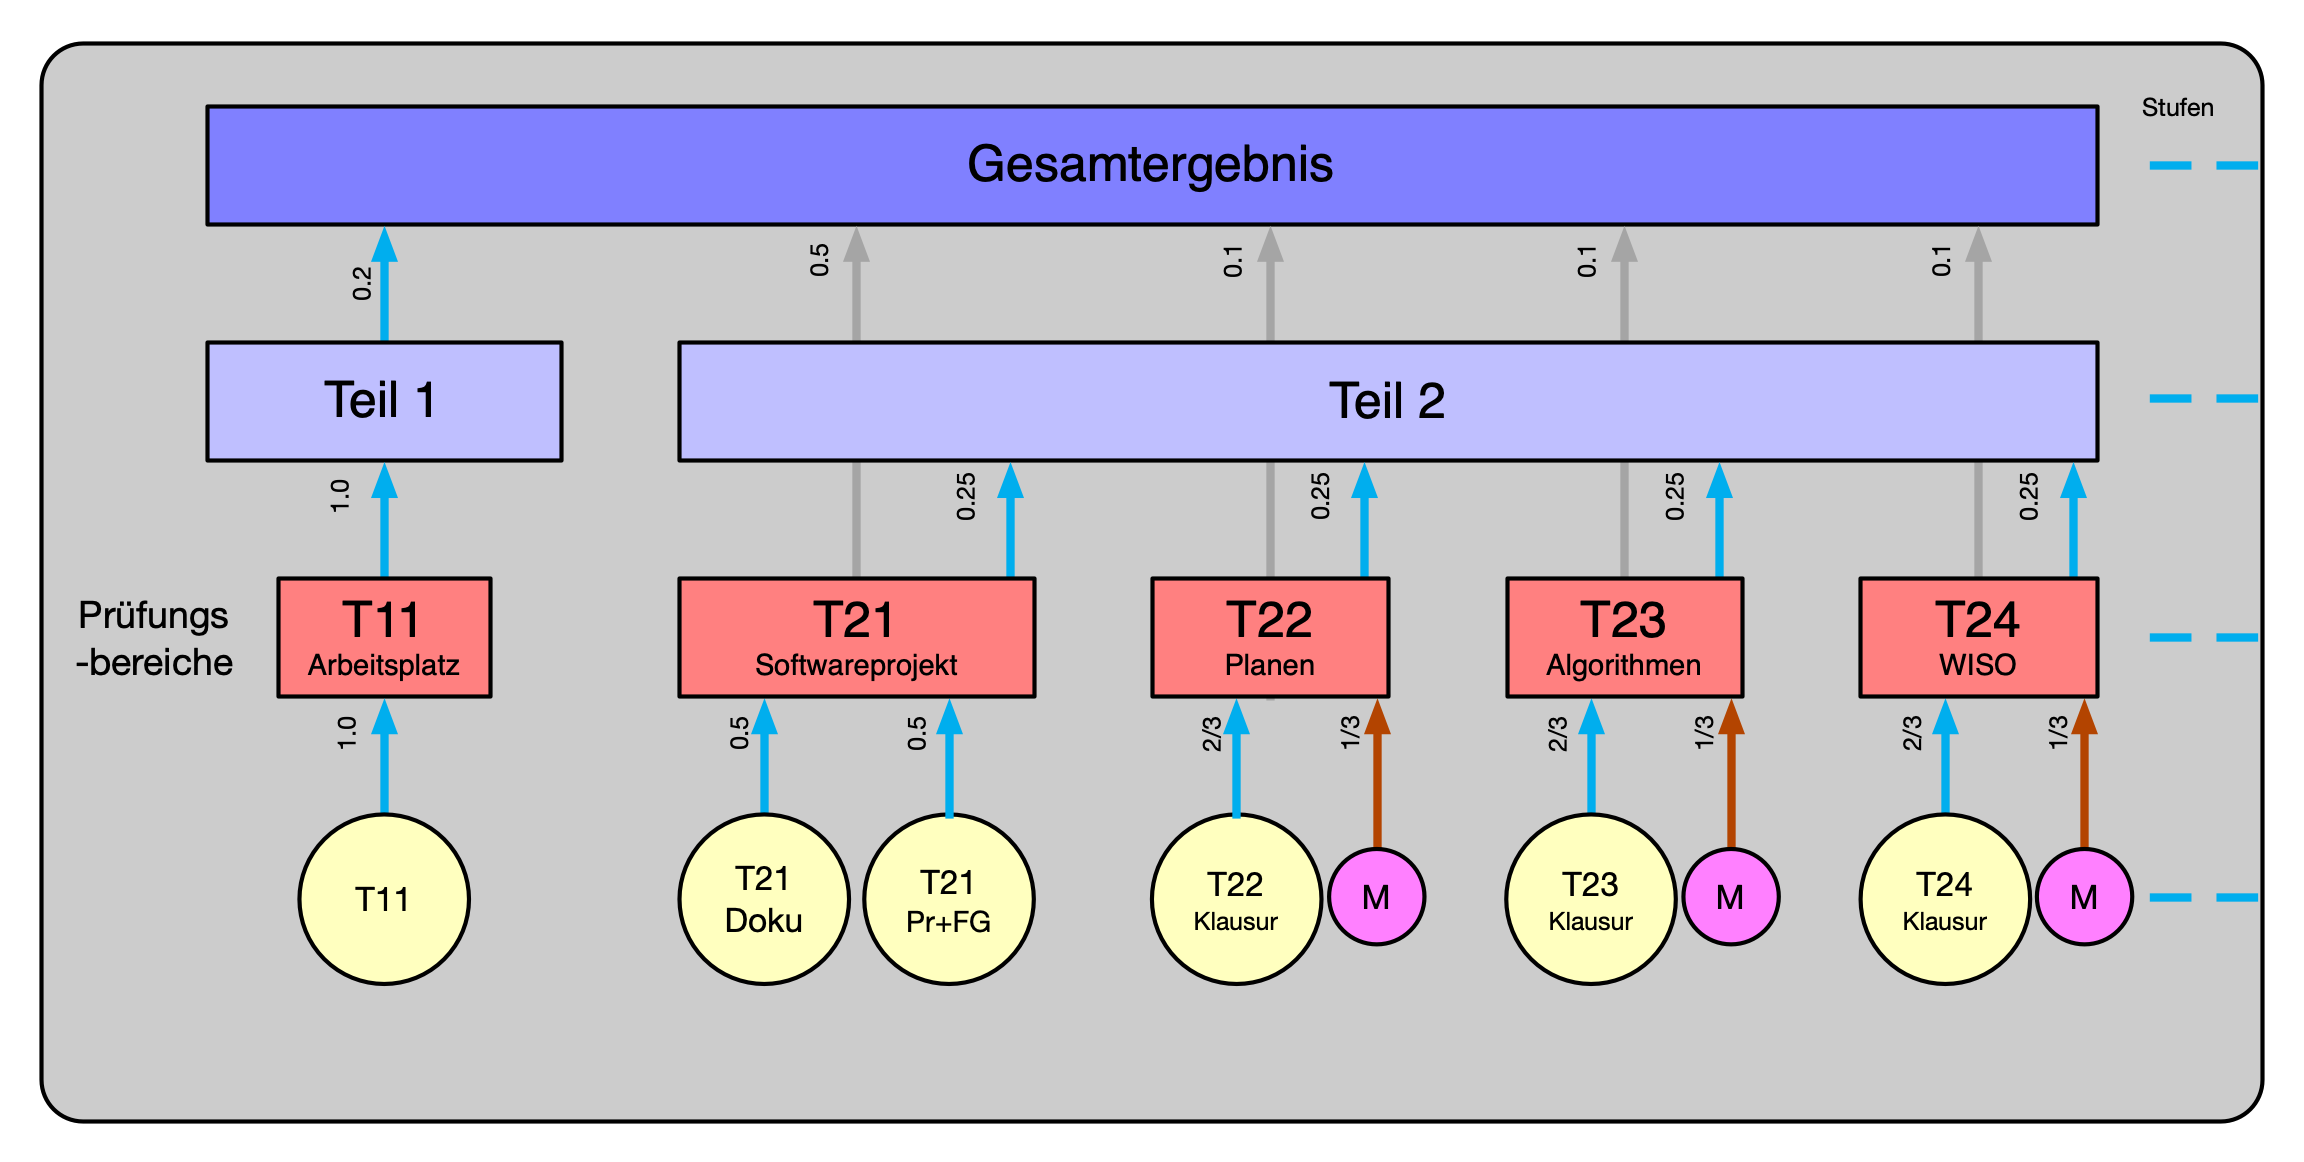
\includegraphics[width=15cm]{FIGrafik.png}
    \caption{Struktur der Prüfung mit Gewichtungen}
    \label{fig:berechnung}
\end{figure}

\section{Funktion des Programms}
Die erste Funktion des Programms ist die Berechnung der Punkte/Noten in den Teilen 1 und 2 der Prüfung und die Berechnung der Gesamtpunktzahl/Gesamtnote.

Dabei ist die Berechnung der Punkte gerade bei einer mündlichen Ergänzungsprüfung (MEPR) von großem Nutzen, da unter dem Zeitdruck einer Prüfung  das Berechnungsverfahren (2:1 Gewichtung) fehleranfällig ist. Man beachte auch, dass der Zeitpunkt der Rundung die Note/Endnote beinflussen kann, daher muss bei jedem Stufenwechsel (s. Abbildung~\ref{fig:berechnung}) auf ganze Zahlen gerundet werden.

Die zweite Funktion des Programms ist eine Simulation der Gesamtergebnisse und der Teilergebnisse in der Teilprüfung T21 (Präsentation und Fachgespräch )  und bei der Vergabe der Punkte in der MEPR (für T22,T23 oder T24).

Mit dieser Simulation ist es leicht möglich, Notengrenzen zu erkennen und ggfs. Notengrenzen bei der Vergabe der Punkte zu beachten. Ein Klick auf diese Notengrenzen überträgt die Punktzahl in die jeweils simulierten Felder (T21b bzw. T2x in der mündlichen Ergänzungsprüfung).

\section{Das Programm}

\begin{figure}[ht]
	\centering
    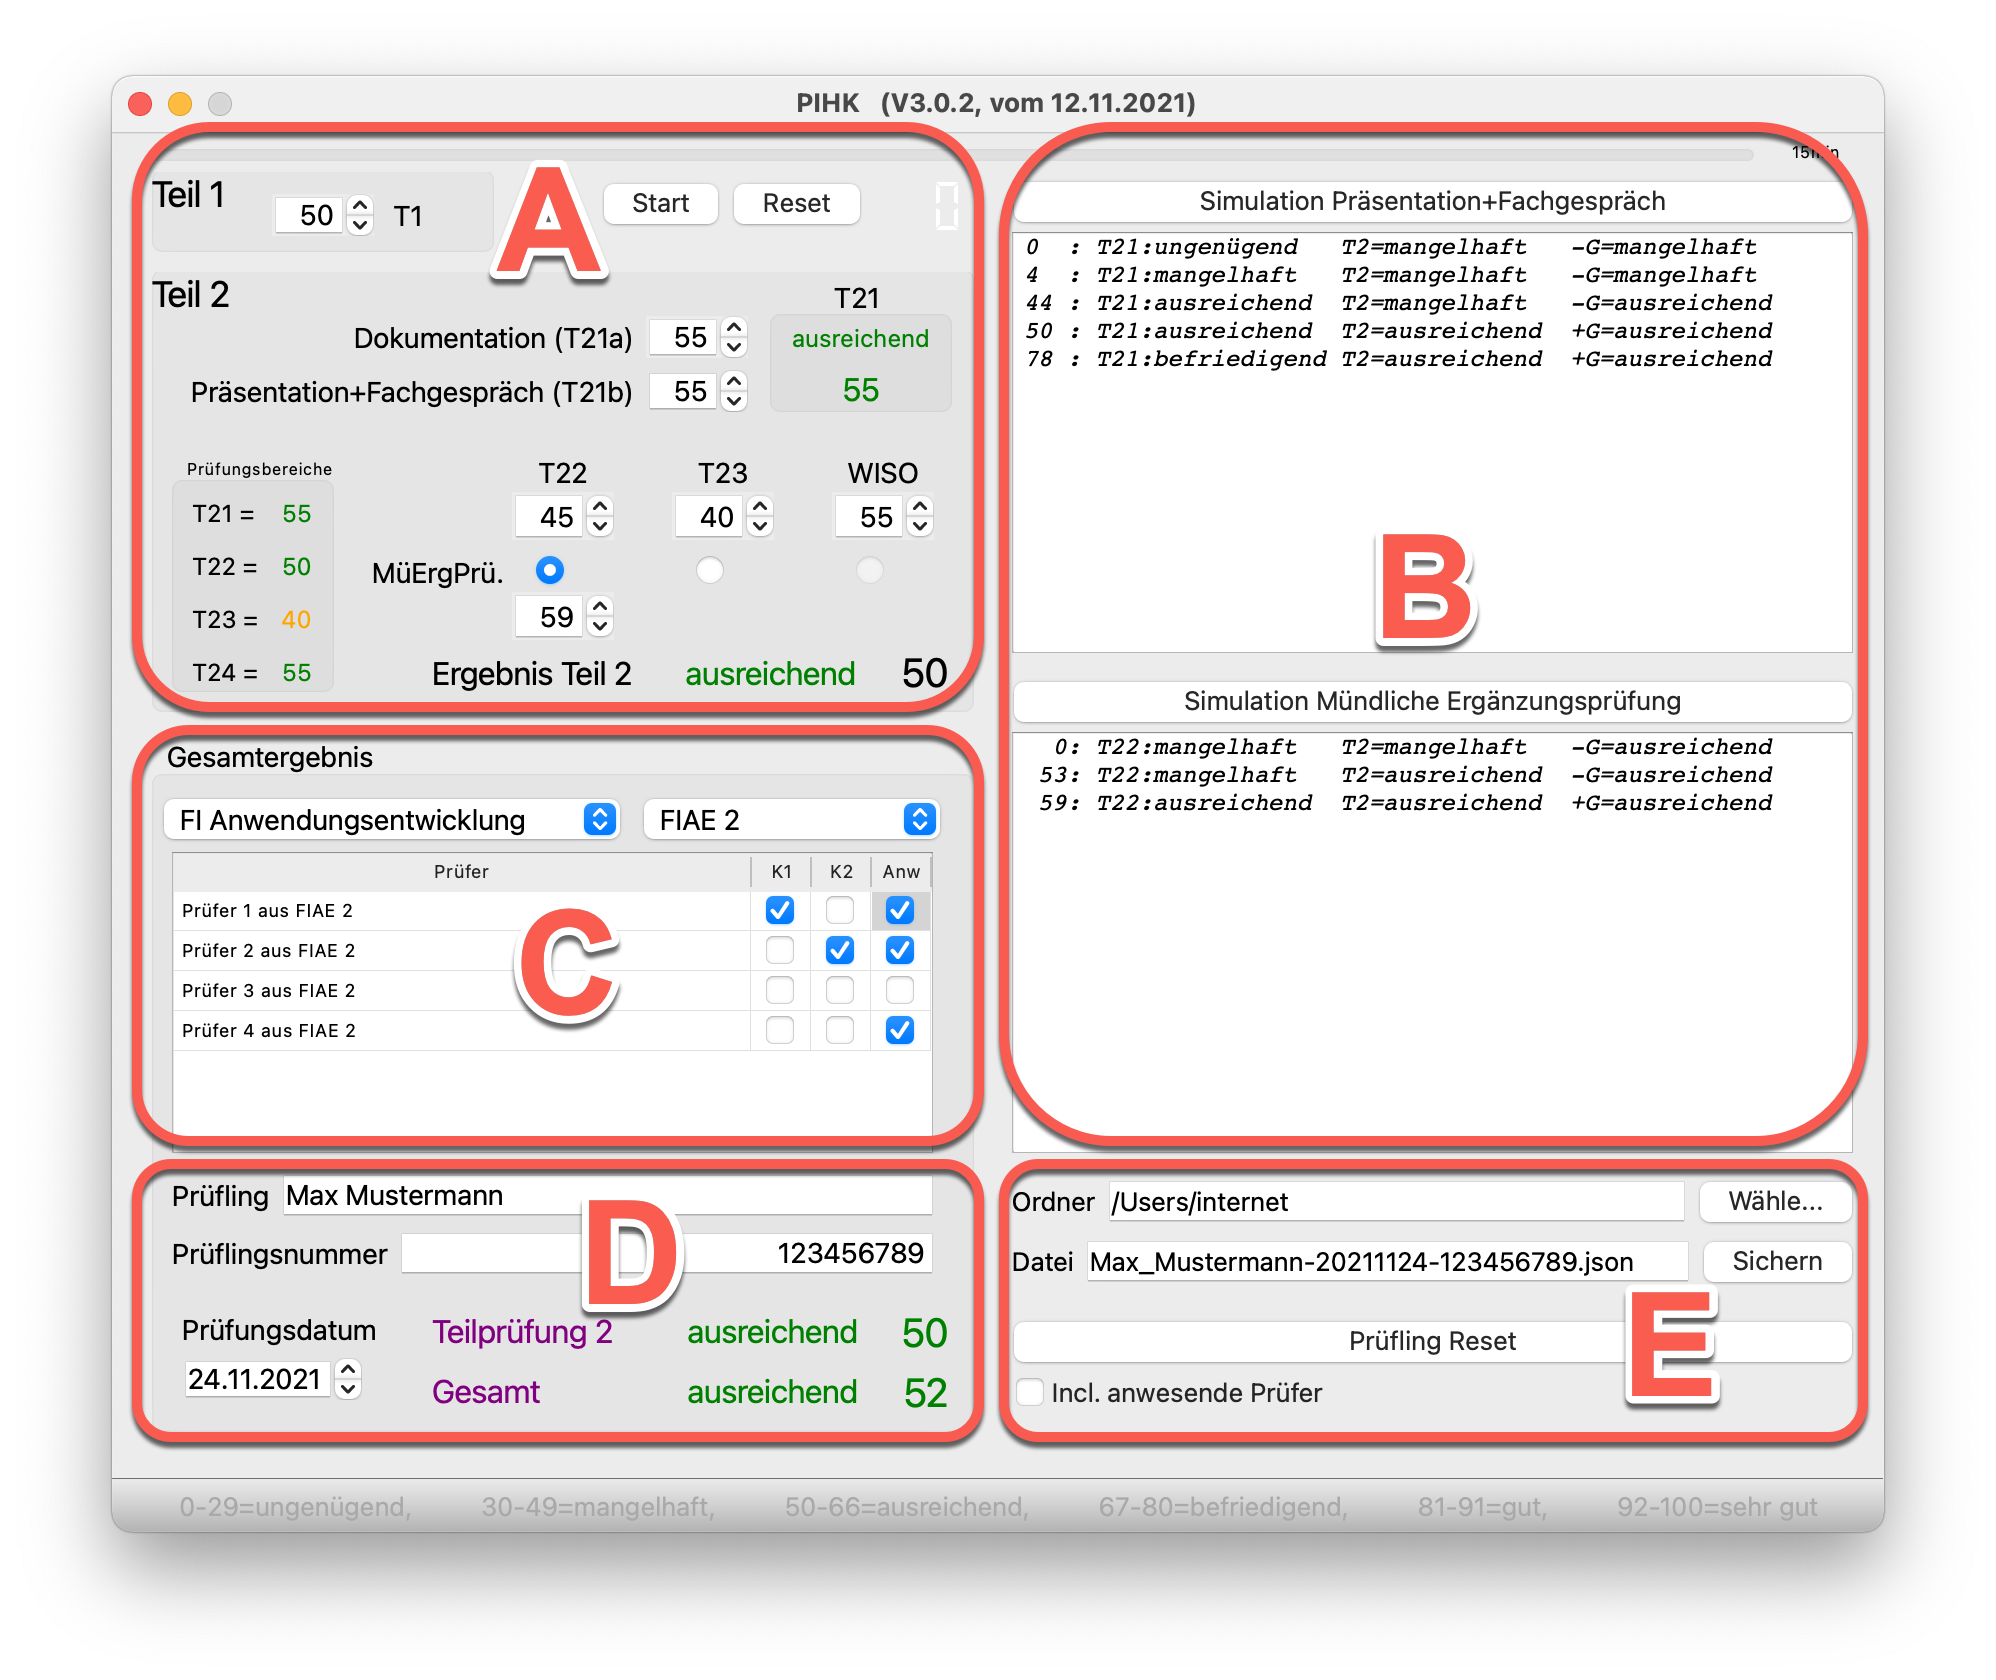
\includegraphics[width=\textwidth]{HauptfensterAufteilung.png}
	\caption{Programmoberfläche -- Bereiche}
	\label{fig:pihk}
\end{figure}

Das Programm (siehe Abbildung~\ref{fig:pihk}) gliedert sich grob in 5 Bereiche (A,B,C,D,E):

\begin{itemize}
\item[(A)] Links oben ist der Bereich zur Eingabe und Berechnung der Punktzahlen und Noten. 
Hier werden alle bisher erreichten Punktzahlen sowie die in der Prüfung erzielten Punkte eingegeben.
Weiterhin beinhaltet dieser Bereich auch einen Timer, mit dem man die Vortragszeit abstoppen kann (wird auf ganze Minute gerundet).
\item[(B)] Rechts oben und in der Mitte befinden sich 2 Fenster zur Anzeige der Simulationsergebnisse.
\item[(C)] Im mittleren linken Bereich kann der Prüfungsausschuss eingegeben werden und die 1. und 2. Korrektoren sowie die anwesenden Prüfer. Die Prüfer und die Ausschüsse, die hier gelistet werden, können im Einstellungsdialog eingegeben werden und werden im System gespeichert (plist bzw. Registry oder ini).
\item[(D)] Im unteren linken Bereich werden Daten zur Prüfung und zum Prüfling eingegeben.
\item[(E)] Im rechten unteren Bereich befinden sich die Funktionen zum Sichern der aktuellen Prüfung und zum Zurücksetzen der aktuellen Prüfung.
\end{itemize} 

\begin{figure}[ht]
    \centering
    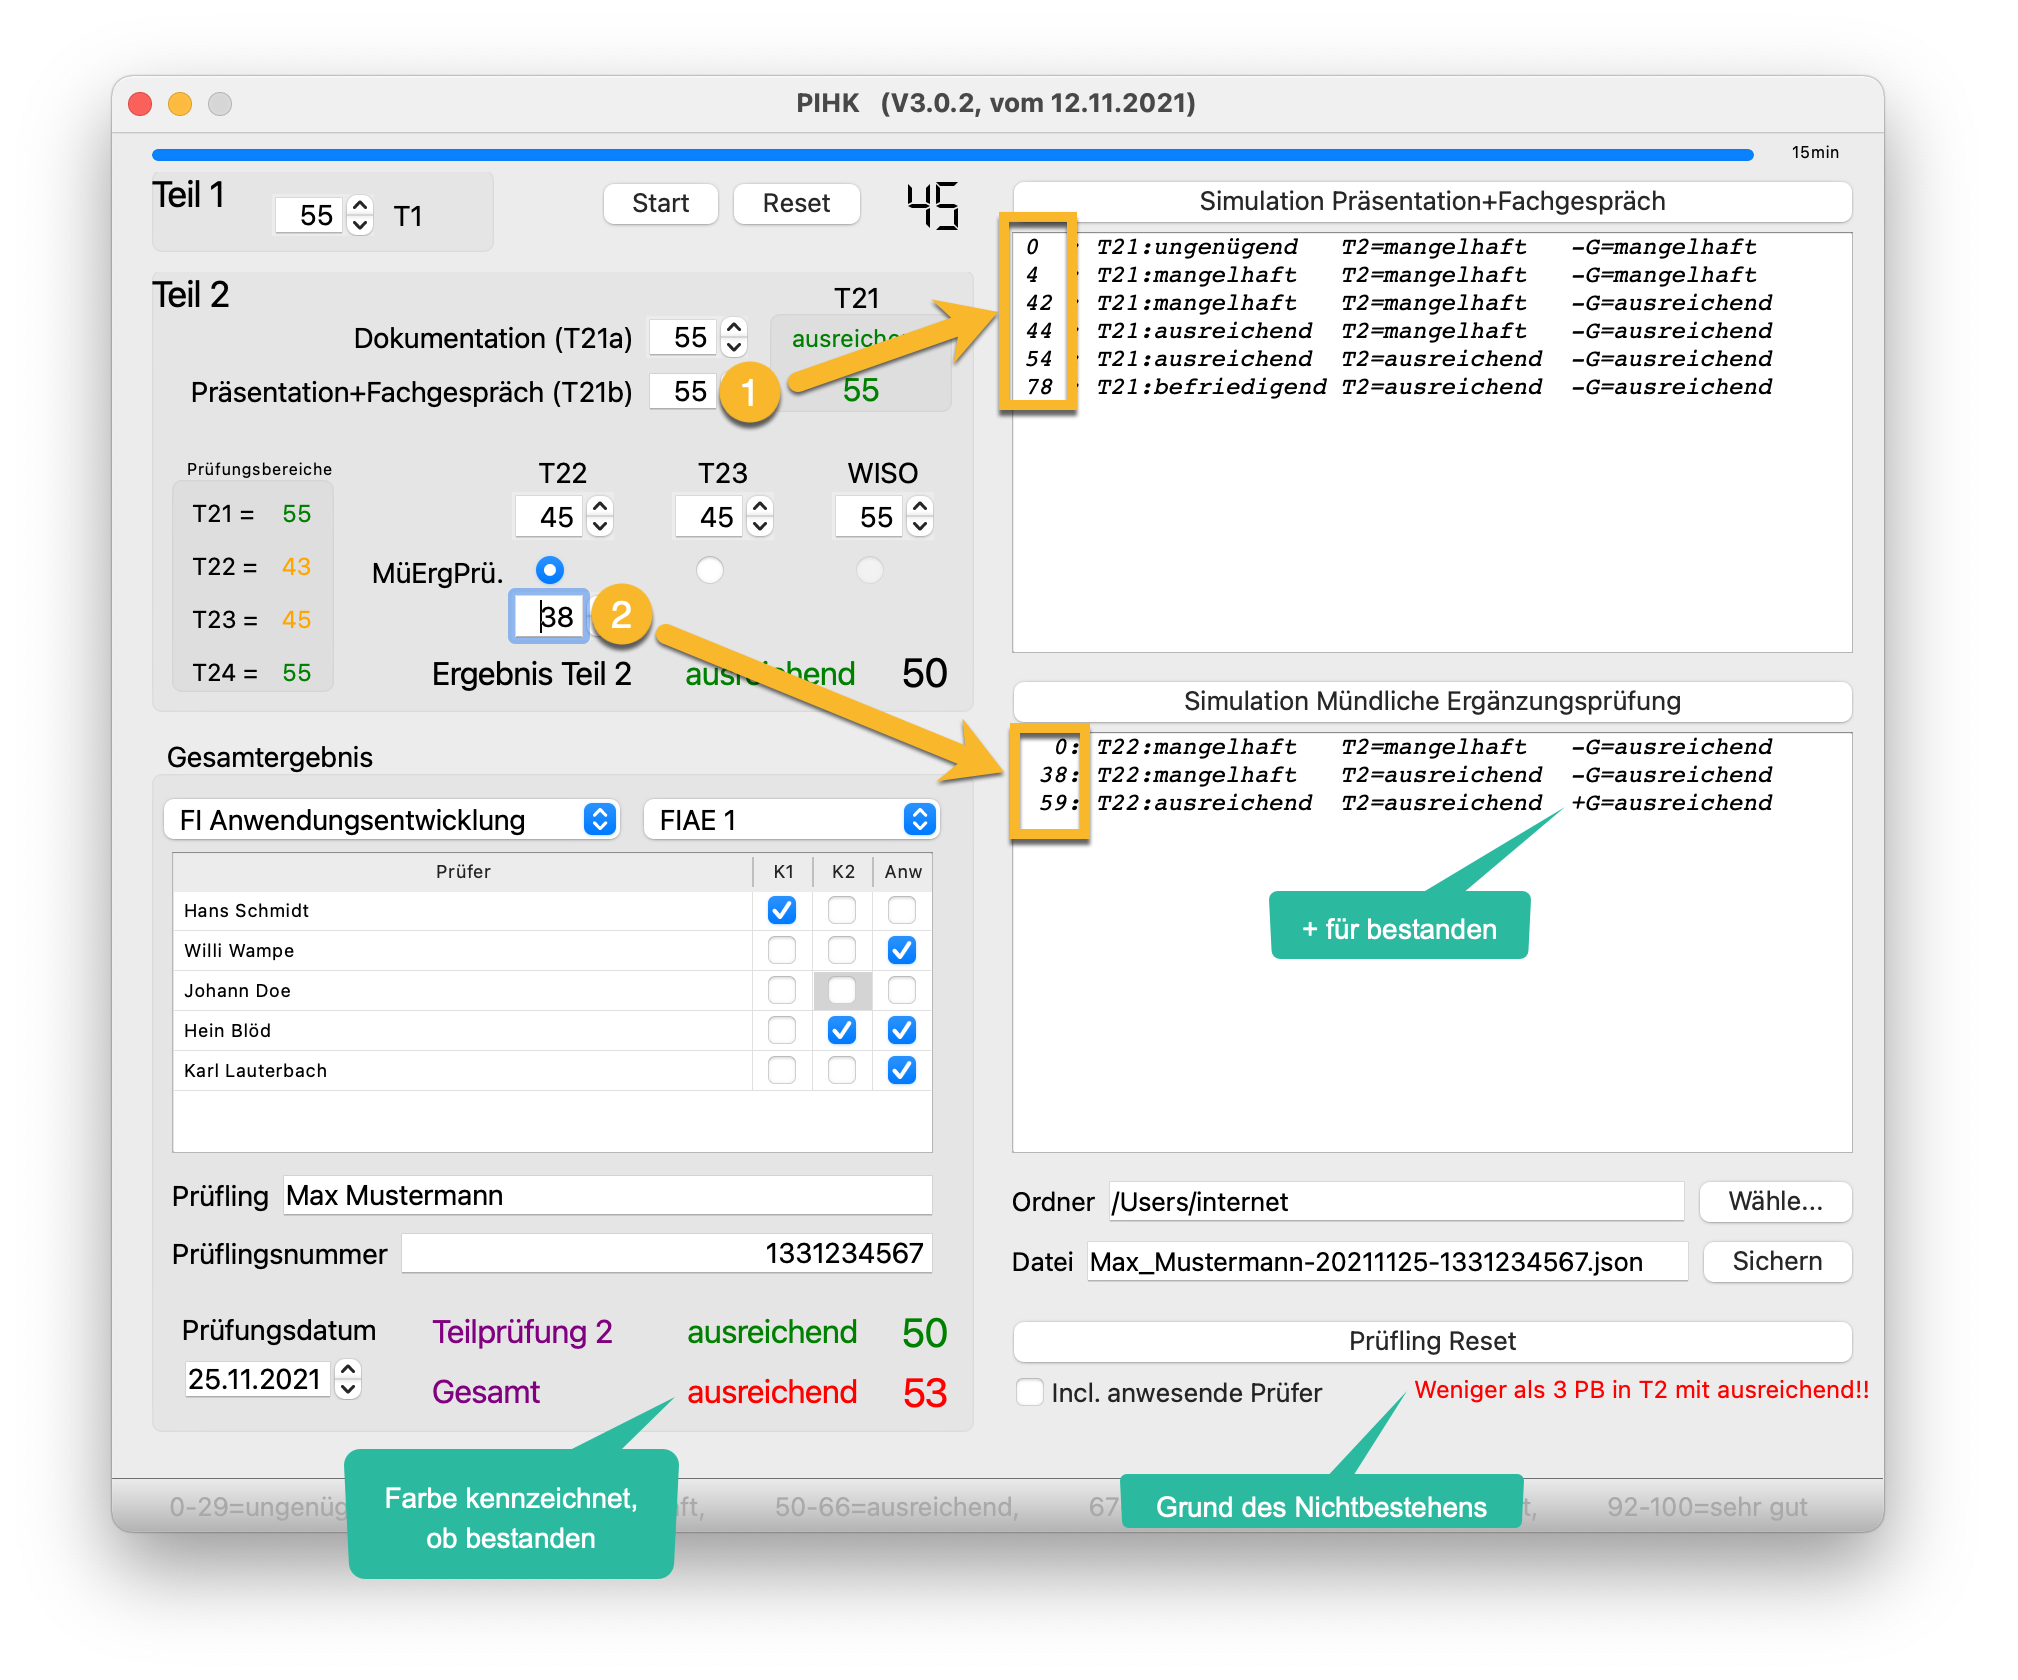
\includegraphics[width=\textwidth]{HauptfensterKommentiert2.png}
    \caption{Programmoberfläche}
    \label{fig:hauptfensterKommentiert2}
\end{figure}

\subsection{Prüfungsbereich Teil 1}
In den oberen Bereich (A) trägt man die Klausurergebnisse für den Teilbereich~1 ein, der mit 20\% in die Gesamtnote eingeht und schon vor der Prüfung bekannt ist.

Dieser Bereich hat keine Relevanz hinsichtlich einer Schwelle für die Bestehensregelung und dient lediglich zur \emph{Anfütterung} von Punkten. Ein \emph{ungenügend} ist hier nicht möglich, denn alle Punkte zählen zu 20\% für die Gesamtnote. Laut Prüfungsverordnung werden zum Bestehen der Gesamtprüfung in diesem Prüfungsbereich keine Anforderungen gestellt.

\subsection{Prüfungsbereich Teil 2}
Der Prüfungteil 2 untergliedert sich in 4 verschiedene Prüfungsbereiche. Zum Bestehen der Gesamtprüfung müssen hier mindestens 3 Prüfungsbereiche mit ausreichend oder besser abgeschlossen werden und in keinem Prüfungsbereich darf ein ungenügend erzielt worden sein.

Der erste Prüfungsbereich T21, bei dem eine Projektarbeit zu leisten ist, ist aufgeteilt in eine Dokumentation T21a (50\%) und eine Präsentation mit anschließendem Fachgespräch (50\%) T21b und ergibt so die Note von T21.

Bei der letzten Prüfung der IHK geht es im wesentlichen um diesen Prüfungsteil. Die anderen Prüfungsbereiche bestehen aus schon absolvierten Klausuren (T22, T23 und T24 (Wiso)). 

\subsubsection*{T21}
Das Ergebnis der Dokumentation liegt in der Regel schon vor und kann im Feld T21a eingetragen werden.
Das Ergebnis der Präsentation zusammen mit dem Fachgespräch wird im Feld T21b eingetragen.
Für dieses Feld wird eine Simulation berechnet und im rechten Simulationsfenster dargestellt.

\subsubsection*{Simulation für das Feld T21b}
Für das Feld \circled{1} in Abbildung\ref{fig:hauptfensterKommentiert2} werden die Punkte simuliert.
Es werden alle möglichen Punktzahlen für die Präsentation+Fachgespräch eingesetzt und nur dann, wenn sich die Note im Teilbereich T21, im Teilbereich 2 oder in der Gesamtbewertung ändert eine Zeile für diese Punktzahl im rechten Simulationsfenster generiert. 

Es gibt auch Fälle, in denen die Punktzahl für die erfolgreiche Gesamtbewertung erreicht ist, aber andere Bedingungen nicht erfüllt sind (z.B. ein Prüfungsbereich mit \emph{ungenügend} bewertet). Diese Fälle werden mit einem Minuszeichen vor dem G in der Simulation gekennzeichnet. Ein Pluszeichen kennzeichnet eine defacto bestandene Prüfung.

Ein Klick auf eine dieser Simulationszeilen befördert die simulierte Punktzahl ganz links in das entsprechende Fenster (T21b) und spart Tipparbeit.
 
\subsubsection*{T22,T23 und T24}
Ebenfalls sind die Klausurergebnisse für die Bereiche T22, T23 und T24 (Wiso) in der Regel schon bekannt und können in die Felder eingetragen werden. 

Falls die Bedingungen für eine mündliche Prüfung vorliegen, kann in den Prüfungsbereichen T22, T23 oder T24 genau eine mündliche Ergänzungsprüfung durchgeführt werden. Sofern dies der Fall ist, werden die Selektoren unter diesen Bereichen aktiviert und können ausgewählt werden (manchmal sind 2 Prüfbereiche für eine mündliche Ergänzungsprüfung möglich und der Prüfling muss sich für einen Prüfungsbereich entscheiden).

Sowie eines der Selektoren ausgewählt ist, erscheint dann ein weiteres Feld zur Eingabe des Ergebnisses der mündlichen Ergänzungsprüfung (MEPR) und wird immer mit 0 initialisiert.

\subsubsection*{Simulation für das Feld T22/T23/T24}
Für das Feld \circled{2} in Abbildung~\ref{fig:hauptfensterKommentiert2} werden die Punkte simuliert.
Für dieses Feld T2x wird auf der rechten Seite ebenfalls eine Simulation berechnet und die Konsequenzen bei den anderen Noten aufgezeigt. Ein Klicken befördert wieder die simulierte Punktezahl in das gewählte Feld T2x.

\subsection{Prüfungsausschuss}
Die Fachrichtung und der Prüfungsausschuss können im Bereich \circled{C} in Abbildung~\ref{fig:pihk} angewählt werden und es erscheint eine Liste der Prüfer.

Diese Prüferliste muss zuvor einmalig in den Einstellungen vorgenommen werden und wird dann beim Verlassen des Programms (optional) abgespeichert und steht dann nächstes mal gleich zur Verfügung (s.~Abschnitt~\ref{sec:einstellungen} auf Seite~\pageref{sec:einstellungen}).

In der Prüferliste kann man duch Anklicken die 1. und 2. Korrektoren auswählen und die anwesenden Prüfer selektieren. Wird dies nicht ordnungsgemäß durchgeführt (z.B. nur 2 anwesende Prüfer oder derselbe Korrektor für 1. und 2. Korrektur, etc.), so erscheint beim Abspeichern später eine Warnmeldung, die man aber auch optional ignorieren kann. Die Daten dienen hier nur zum Erfassen der vollständigen Prüfungsdaten beim Abspeichern als \emph{JSON}--Datei. 

\subsection{Prüfungsinformationen}
Links unten in Abbildung~\ref{fig:pihk} im Bereich \circled{D} findet man Angaben zur Prüfung, wie Datum der Prüfung , Name und Nummer des Prüflings.

Hier werden auch die relevanten Prüfungsergebnisse dargestellt.

Zu beachten ist noch, dass es Situationen geben kann, die zwar hinreichend viele Punkte im Teil~2 oder der Gesamtnote liefern, aber wegen des Fehlens einer weiteren Bedingung zu einem Nichtbestehen der Prüfung führen.

In einem solchen Fall ist die entsprechende Note zwar \emph{ausreichend} oder besser, aber die Farbe ist \emph{rot}. Gleichzeitig wird die entsprechende Bedingung in rot im Bereich \circled{E} angezeigt (s. Abbildung~\ref{fig:hauptfensterKommentiert2}).

\subsection{Speichern und Zurücksetzen}
Im Bereich \circled{E} kann die Prüfung abgespeichert und resettet werden.

Die Angaben aus den Prüfungsinformationen können dazu benutzt werden, um einen eindeutigen Dateinamen zu generieren, der unten rechts immer angezeigt wird und beim Sichern benutzt wird. 

Werden für den Dateinamen Zeichen benutzt, die auf bestimmten Plattformen Probleme bereiten könnten, so wird eine Warnung ausgegeben, die aber optional ignoriert werden kann. 

Der aktuelle Ordner kann dabei mit dem \button{Wähle...}--Button eingestellt werden.

Der \button{Sichern}--Button sichert die Datei mit dem eingestellten Muster für den Dateinamen (s.a. Abschnitt \emph{Einstellungen}) und wird anschließend deaktiviert. Erst bei Änderungen wird dieser Button wieder aktiviert.

Die gemachten Einstellungen zum Dateinamen und zum Ordner werden beim Beenden des Programms (optional) abgespeichert und stehen beim nächsten Start sofort wieder zur Verfügung.

Folgende Daten werden beim Verlassen des Programms im Hintergrund abgespeichert:
\begin{enumerate}
\item Dateinamensmuster inklusive der Trennzeichen und das Ersetzungszeichen für Leerzeichen.
\item Die Länge der Prüfung in Minuten.
\item Der Ordner, in den die Dateien gespeichert werden und der mit dem \button{Wähle...} Button ausgewählt wurde.
\item Die Struktur der Fachrichtungen, Ausschüsse und die Prüferlisten
\item Die aktuell angewählte Fachrichtung und Prüfungsausschuss
\end{enumerate}
 
\subsection{Timer}
Mit dem Timer hat man die Möglichkeit, die Vortragslänge abzustoppen.
Die Länge des Timers kann im Einstellungsdialog von 1 bis 99 eingestellt werden und ist anfänglich auf 15 Minuten eingestellt.

Bei Überschreiten der eingestellten Zeit beginnt der Zähler wieder bei 0 und man kann direkt die überzogene Zeit ablesen.

Der Timer kann jederzeit durch \button{Stop} unterbrochen werden und durch \button{Start} wieder gestartet werden. Mit \button{Reset} setzt man den Timer wieder zurück.

\section{Einstellungen}
\label{sec:einstellungen}
\begin{figure}[ht]
  \centering
  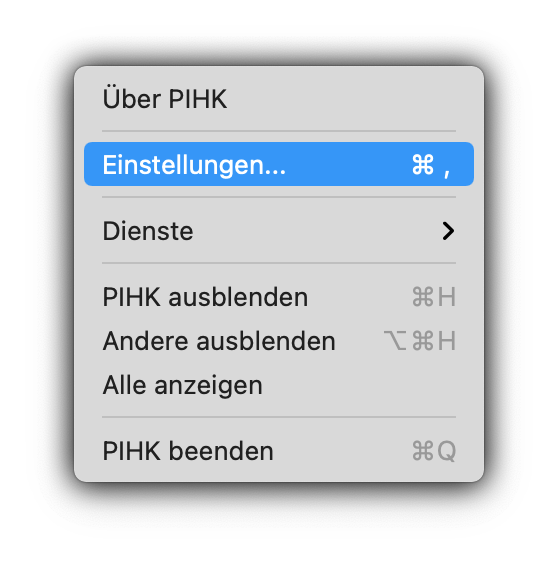
\includegraphics[width=0.3\textwidth]{menu0.png}
  \caption{Das Einstellungsmenü}
  \label{fig:menu}
\end{figure}

Der Einstellungsdialog wird durch einen entsprechenden (Applikations--)Menüeintrag (\emph{macOS}) bzw. im Datei--Menü (\emph{Windows}) angezeigt.

\begin{figure}[ht]
  \centering
  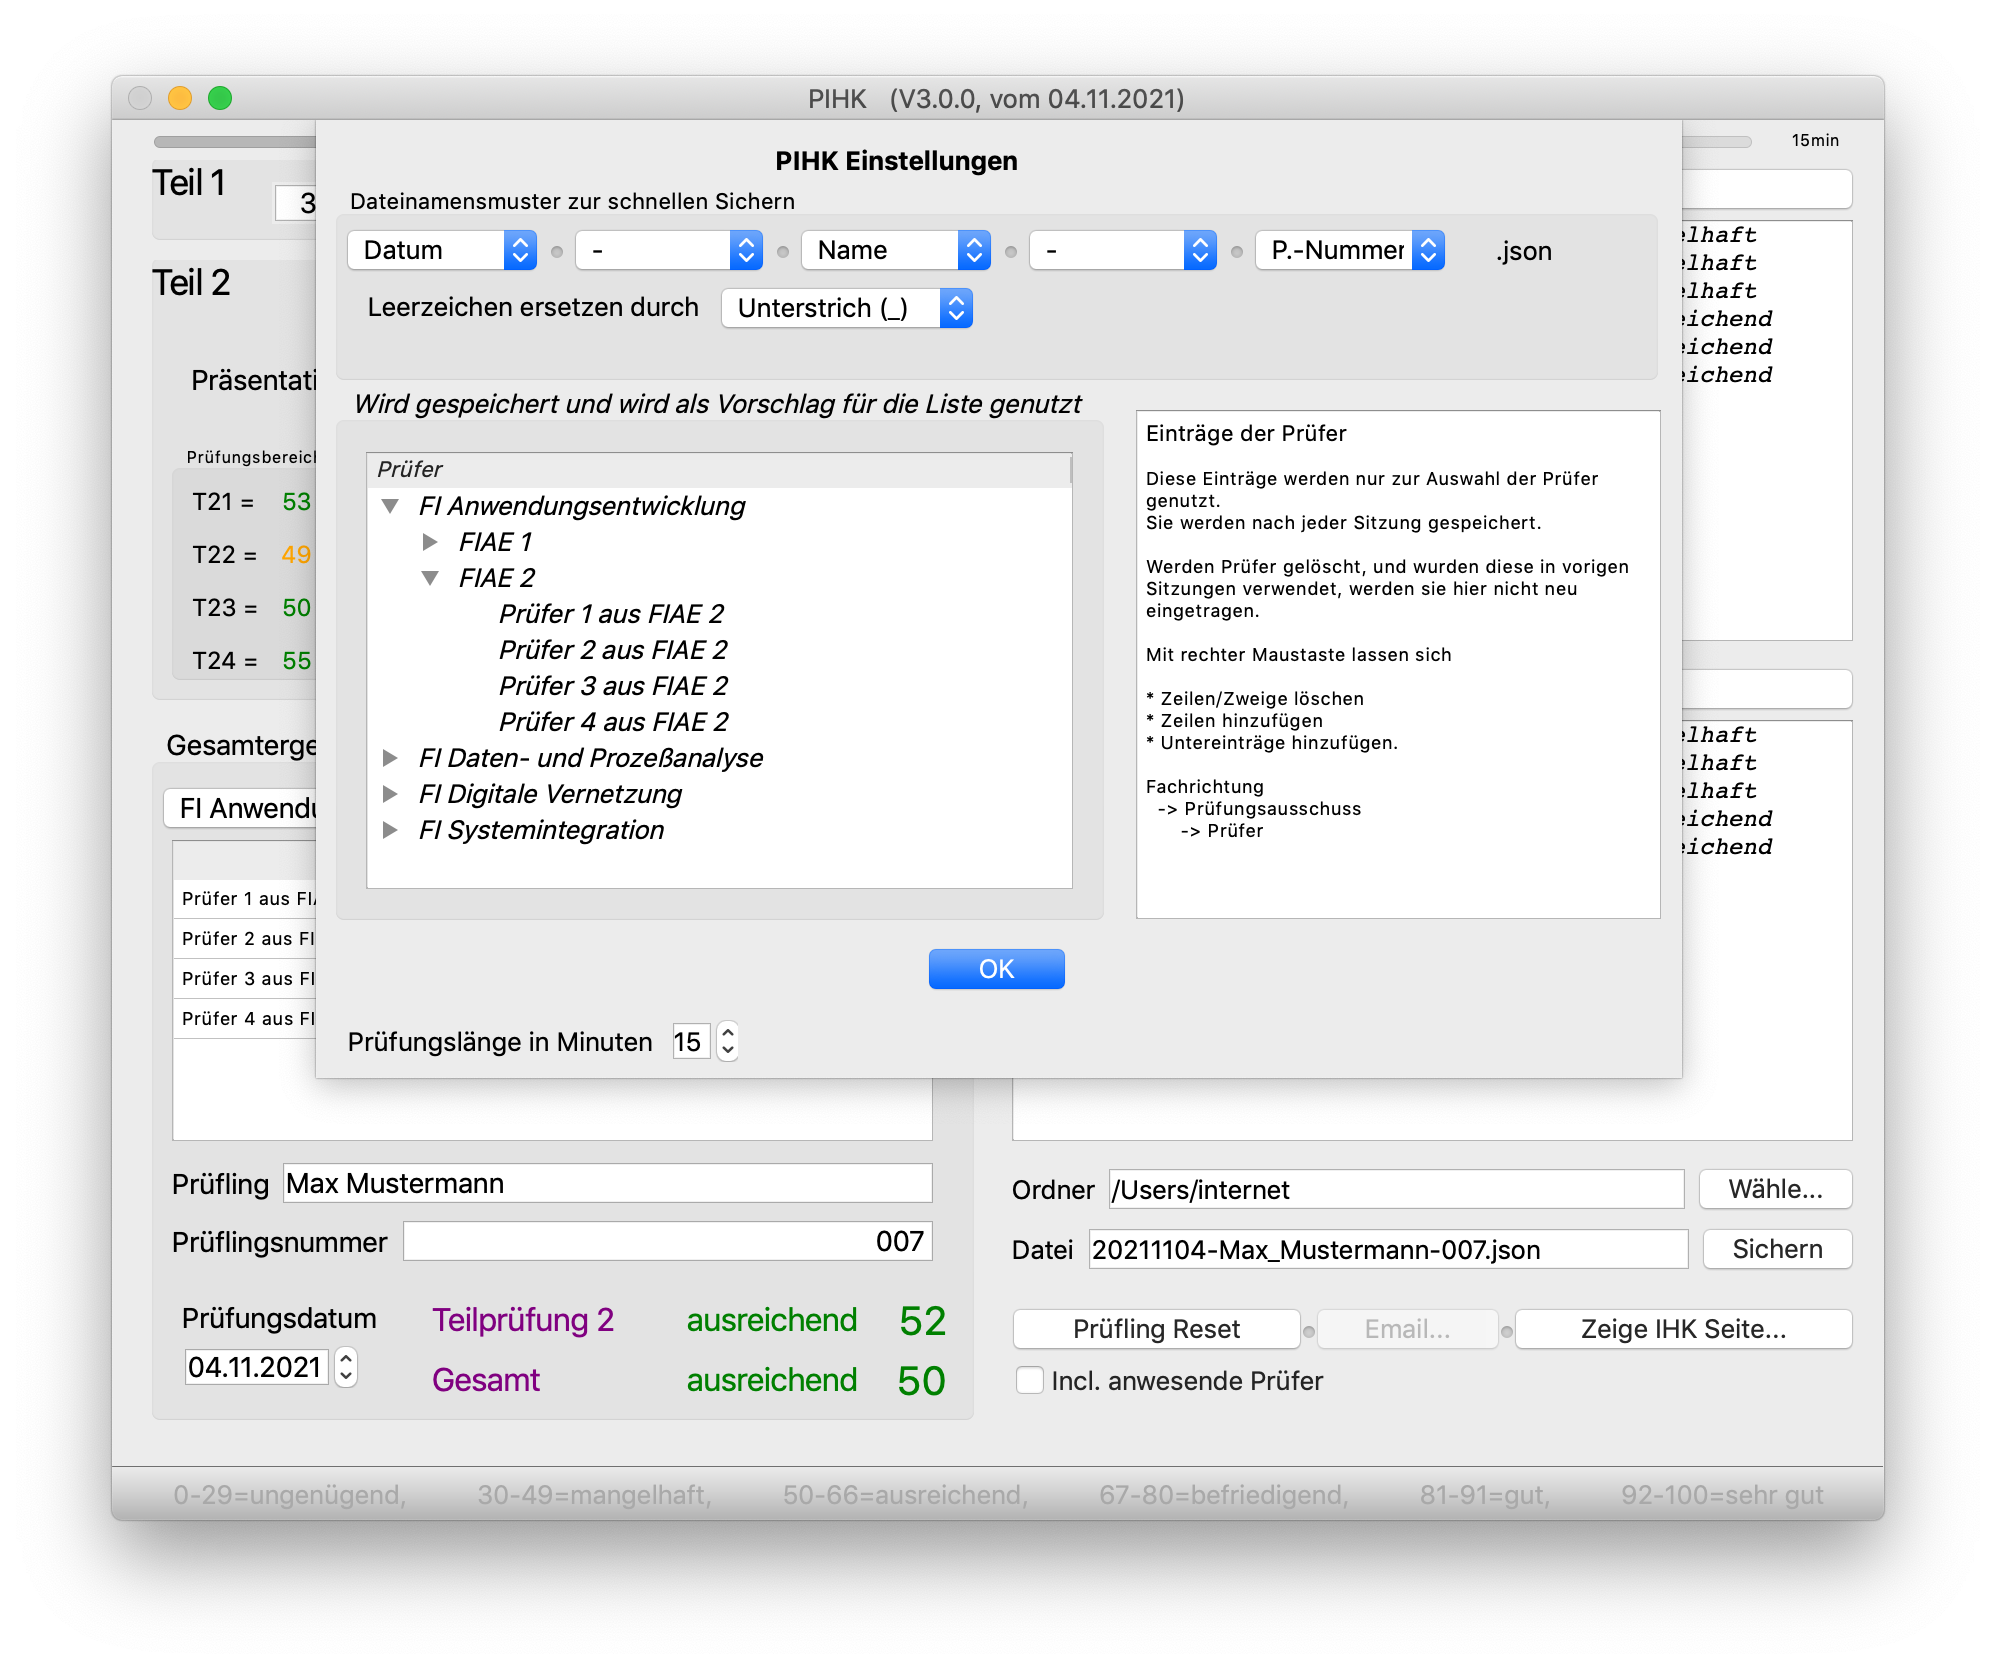
\includegraphics[width=\textwidth]{Einstellungen.png}
  \caption{Einstellungen}
  \label{fig:einstellungen}
\end{figure}


Achtung: Änderungen in diesem Einstellungsdialog sind \emph{immer sofort gültig} und die alten Werte werden nicht zwischengespeichert.

\subsection{Namensmuster}
Hier kann man das Namensmuster des Dateinamens einstellen und die Trennzeichen im Namen definieren.

Dadurch erhält man einen konsistenten und eindeutigen Dateinamen und muss später nur noch auf den \button{Sichern}--Button drücken, um die aktuelle Prüfung abzuspeichern.

Das Muster für den Dateinamen und die Trennzeichen werden beim Verlassen des Programms (optional) gesichert.

\subsection{Prüfungszeit}
Unten links kann man die Prüfungszeit im Bereich von 1 bis 99 Minuten verändern, was aber im Normalfall nicht notwendig sein sollte. Der Wert wird beim Verlassen des Programms (optional) gesichert.

\subsection{Eintrag der möglichen Prüfer}
Im Einstellungsdialog wird auch die Liste der Prüfer gepflegt, die später angezeigt werden können und aus denen pro Prüfung die jeweiligen Korrektoren ausgewählt werden können.

Dazu klickt man mit der rechten Maustaste auf einen vorhandenen Eintrag und es öffnet sich ein Kontextmenü.

Nun kann man entweder

\begin{itemize}
\item eine Zeile hinzufügen,
\item die aktuelle Zeile löschen oder
\item eine Unterkategorie einfügen. 
\end{itemize}

\begin{figure}[ht]
  \centering
  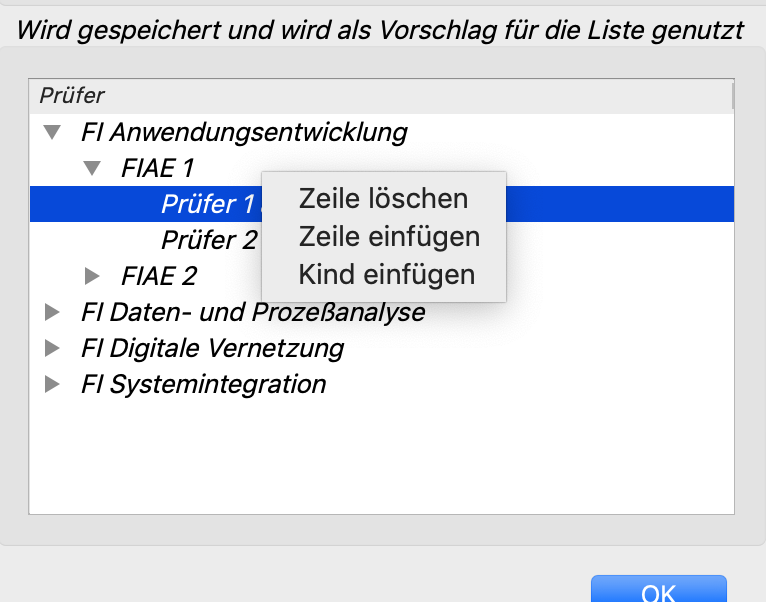
\includegraphics[width=0.5\textwidth]{Einstellungen2.png}
  \caption{Einpflegen der Prüfer}
  \label{fig:einstellungen2}
\end{figure}

Den Platzhaltertext der neuen Zeile kann man dann löschen und eigenen Text einfügen.

\begin{marker}
Das Programm erwartet auf der ersten Ebene immer die Fachrichtung, als 2. Ebene einen Prüfungsauschuss und als 3. Ebene den Namen des Prüfers. Weitere Ebenen können hinzugefügt werden (z.B. Kontaktdaten,etc.) werden aber nicht angezeigt und ausgewertet.
\end{marker}

Das Programm ist nicht vollständig sicher gemacht und scheitert bei unsinnigen Eingaben.

In der Regel muß auch nur der Prüfungsausschuss umbenannt werden oder neu eingefügt werden und die Prüfer müssen eingetragen werden. Auf der Ebene der Fachrichtung sollten keine Änderungen notwendig werden.

Auch wenn eine Prüfung abgespeichert wird und später diese Daten im Prüfungsauschuss gelöscht werden und dann diese Datei wieder geladen wird, kann zwar der Name eines unbekannten Prüfers wieder eingefügt werden, aber gelöschte Prüfungsausschüsse dürften zu Problemen führen.

\section{Benutzung}

Ein empfohlener Arbeitsfluss:

\begin{enumerate}
\item Erstmalig im Einstellungsdialog den Prüfungsausschuss eintragen und mit Namen des Ausschusses und der Prüfer füllen.
\item[1] Im Einstellungsdialog das Dateinamensmuster definieren, um die gesicherten Dateien gut zu beschreiben.
\item[2] Im Hauptfenster den Prüfungsausschuss wählen (es erscheinen die Prüfer)
\item[3] Anwesende Prüfer und 1.-- und 2.--Korrektoren wählen
\item[4] Prüfungsdatum, Name des Prüflings und ggfs. Nummer eintragen
\item[5] (Optional) Eigenen Ordner für Prüfungdateien erzeugen/wählen
\item[6] T1, T21a, T22,T23,T24 eintragen
\item[7] Nach Fachgespräch (unter Berücksichtigung der Simulation) die Punkte in T21b eintragen.
\item[8] Bei möglicher MEPR: Prüfungsbereich anwählen und (Simulation!) Punkte eintragen T2x
\item[9] Am Ende auf den \button{Sichern}--Button drücken und die Daten werden als JSON--Datei abgespeichert.
\item[10] Ein Reset der Prüfungsdaten durchführen (standardmäßig bleiben die anwesenden Prüfer eingetragen).
\item[11] Weiter bei Punkt 4
\end{enumerate}

\section{Ausgabe}
Die \emph{JSON}--Datei, die gespeichert wird, hat folgenden Inhalt (im Original alphabetisch sortiert):
\nopagebreak[4]

\begin{minipage}[t]{\textwidth}
\begin{lstlisting}[numbers=none,caption={\cfile{Gesicherte Datei: $20160621Max\_Mustermann13145678.txt$}},label=lst:datei]
{
    "Fachrichtung": "FI Anwendungsentwicklung",
    "Ausschuss": "FIAE 2",
    "Anwesend": [
        "Prüfer 1 aus FIAE 2",
        "Prüfer 2 aus FIAE 2",
        "Prüfer 4 aus FIAE 2"
    ],
    "Korr1": [
        "Prüfer 1 aus FIAE 2"
    ],
    "Korr2": [
        "Prüfer 2 aus FIAE 2"
    ],
    "Datum": "01.11.2021",
    "Doku": "61",
    "PRFG": "44",
    "GA0": "39",
    "GA1": "49",
    "GA2": "44",
    "Wiso": "55"
    "MEP-GA1": "0",
    "MEP-GA2": "61",
    "MEP-WISO": "0",
    "Name": "Max Mustermann",
    "Id-Nummer": "007",
    "Ergebnis B": " 52 ( ausreichend)",
    "Ergebnis": " 50 ( ausreichend)",
    "Prüfungsergebnis": "NICHT bestanden",
    "Prüfungszeit": 0,
    "PIHKVersion": "3.0.2",
}


\end{lstlisting}
\end{minipage}

\section{Ansicht}
\subsection{Bericht}
Im Menü \emph{Ansicht} findet man die Funktion \framebox{Bericht...}.
Hier kann man eine Datei angeben (Default: \texttt{Report.pdf}), die aus allen JSON--Dateien im angegebenen Ordner erzeugt wird und eine Zusammenfassung der Ergebnisse enthält (s. Abbildung~\ref{fig:bericht}).

Die Liste enthält dann

\begin{enumerate}
 \item Name des Prüflings
 \item Prüfungsnummer
 \item BESTANDEN/NICHT bestanden
 \item Datum der Prüfung
 \item Punkte im Teilbereich 2
 \item Gesamtpunkte
 \item T1, T21, T22, T23, T24 und ggfs. eine mündliche Ergänzungsprüfung
 \item 1. und 2. Korrektoren
 \item Anwesende Prüfer
 \end{enumerate} 

\begin{figure}[ht]
  \centering
  \framebox{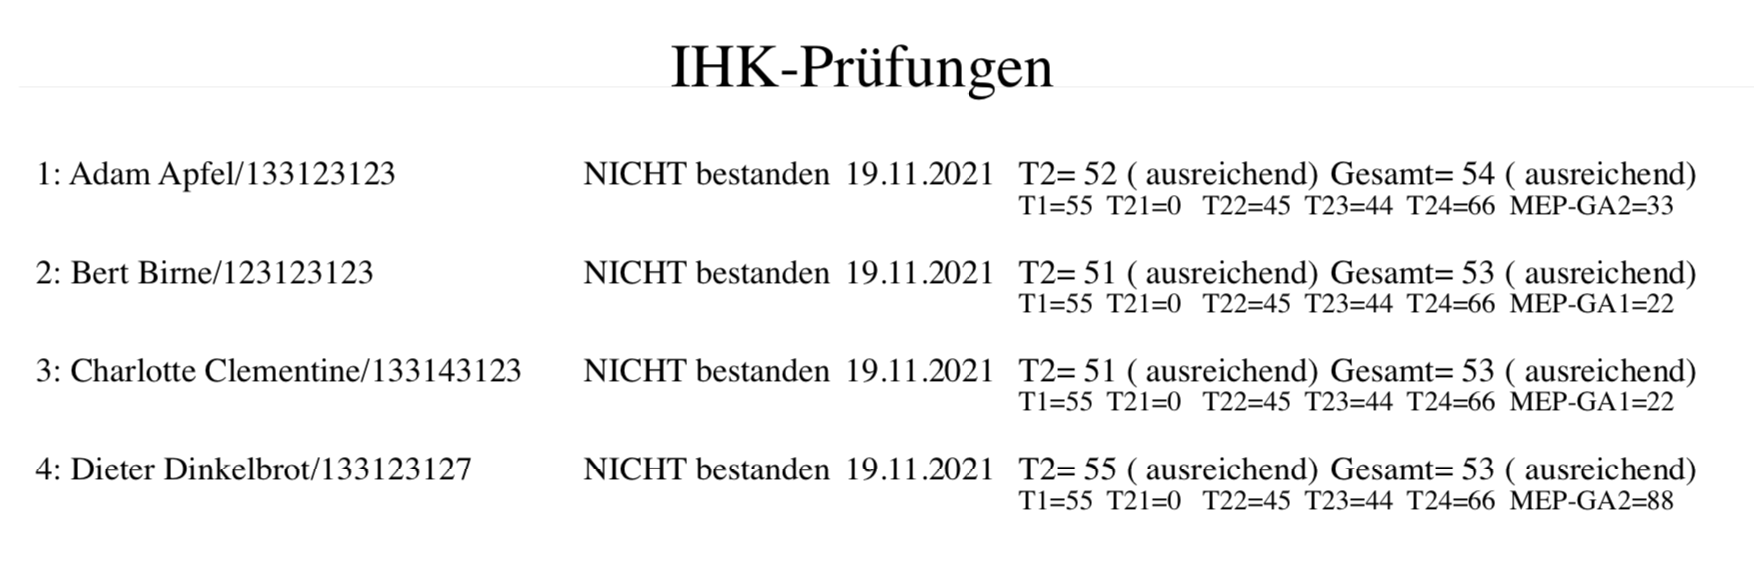
\includegraphics[width=0.9\textwidth]{Bericht.png}}
  \caption{Bericht der Prüfungen im gewählten Ordner}
  \label{fig:bericht}
\end{figure}

\section{Hilfen}
Im Menü \emph{Hilfe} findet man neben der Lizenzvereinbarung (LGPL3) auch die aktuelle Version der Prüfungsordnung
(Verordnung über die Berufsausbildung zum Fachinformatiker und zur Fachinformatikerin* (Fachinformatikerausbildungsverordnung - FIAusbV)), mit deren Hilfe man strittige Fälle leichter klären kann.

\section{Plattform}
Das Programm wurde sowohl für Microsoft Windows als auch für Apple OSX programmiert und steht für beide Plattformen zur Verfügung. 

Entwickelt wurde das Programm hauptsächlich auf macOS 10.14.

Getestet  wurde für MS Windows auf Win~10/11 und für Apple~OSX auf Mojave(10.14) und Big Sur(11.x).
Es wird für MS~Windows als \texttt{.exe} und für Apple~OSX als \texttt{.dmg} Datei zur Verfügung gestellt. 

\section{Programmpflege}
Das Programm wurde ohne finanzielles Interesse zur Erleichterung der eigenen Arbeit im Prüfungsausschuss erstellt.

Das Programm kann von anderen frei genutzt werden, eine Verantwortung zur Pflege des Programms erwächst dem Autor deshalb nicht.

Sollten dem Autor Fehler gemeldet werden, so werden diese \emph{nach Möglichkeit} korrigiert. Hinweise und Fehler sollten per Email an die hier angegebene Adresse gesendet werden.

Das Programm wurde erstellt von:

Frank Zimmermann\\
fz@zenmeister.de

Es sei darauf hingewiesen, dass die IHK--Hannover keinerlei Verantwortlichkeiten für dieses Programm besitzt.
\section{Änderungshistorie}
\begin{table}[H]\centering
\begin{tabular}{|l|l|r|}
\hline
Datum & Änderung &Version\\
\hline
01.12.2021&	Fehlerberichtigungen, Berichtsfunktion	&  3.0.3\\
11.11.2021& Anpassung an neue Prüfungsordnung &  3.0.2\\
11.2.2020&	Windows Version						&  2.2.0\\
4.7.2016&	Initiale, ungetestete Version		&  2.1.0\\
23.6.2016&	XPlattform-Version, doppelte Rundung&  2.0.1\\
04.7.2016&	Klick in Simulation trägt Punkte ein&  2.0.2\\
\hline
\end{tabular}
\caption{Änderungshistorie}
\end{table}

\begin{marker}
In der heutigen Zeit verlangen viele Platformen eine relativ teure Registrierung für Entwickler, damit die Programme leicht auf den Platformen installiert werden können (Signierung/Notarisierung). Erfolgt keine Signierung und Authentfizierung melden die Platformen standardmäßig i.a. gefährlichen Code!. Dieses Programm enthält keinen Schadcode und kann problemlos geöffnet werden.
Erhältlich ist das Programm entweder direkt vom Autor oder über die Github--Seite.
Das Programm kann auch gegen einen Hashcode verglichen werden, was das Risiko weiter minimiert.
Da das Programm aber hauptsächlig zur eigenen Verwendung geschrieben wurde, wird auf eine Signierung und Notarisierung verzichtet.

Bei macOS kann man erstmalig in das Programm--Verzeichnis gehen und mit Öffnen des Kontextmenüs auf das Programm PIHK bestätigen, dass man dieses Programm öffnen möchte.
Bei weiteren Starts wird dann keine Abfrage mehr vorgenommen. (Ein Doppelklick führt dagegen nur zu einer Sicherheitswarnung, die es verbietet dieses Programm zu öffnen).
Bei Windows gibt es ähnliche Sicherheitsvorkehrungen, die man aber durchaus auch umgehen kann, wenn man der Quelle vertrauen schenkt.
\end{marker}

\end{document}